\documentclass{standalone}
\usepackage{tikz}
\usetikzlibrary{intersections}

\begin{document}
	\begin{tikzpicture}[line width = 0.3mm]
	
	\node[anchor = center, inner sep = 0, outer sep = 0] (I) at (0, 0) {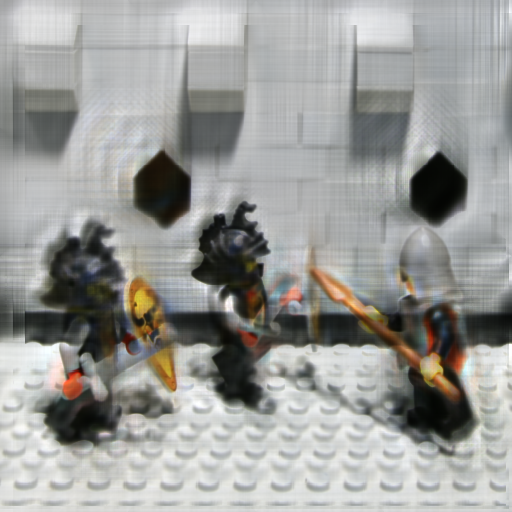
\includegraphics[width = 3.75cm]{../Figures/depth_compression/baseline_unscaled/Reconstruction_of_view_(9,9).png}};
	
	\coordinate (A1) at (-0.6, -1.7);
	\coordinate (S1) at (1, 1);
	\coordinate (A2) at (-1.7, 0.2);
	\coordinate (S2) at (1, 1);
	
	\draw[red]  (A1) rectangle ++(S1); 	
	\draw[blue] (A2) rectangle ++(S2); 
	
	% Magnification box 1
	\node[anchor = south west, xshift = 0.1cm, inner sep = 0pt, outer sep = 0pt, scale = 1.825] (box1) at (I.south east) {
		
		\begin{tikzpicture}
			\begin{scope}
				\clip(A1) rectangle ++(S1);
				\node[anchor = center, inner sep = 0pt] (I) at (0, 0) {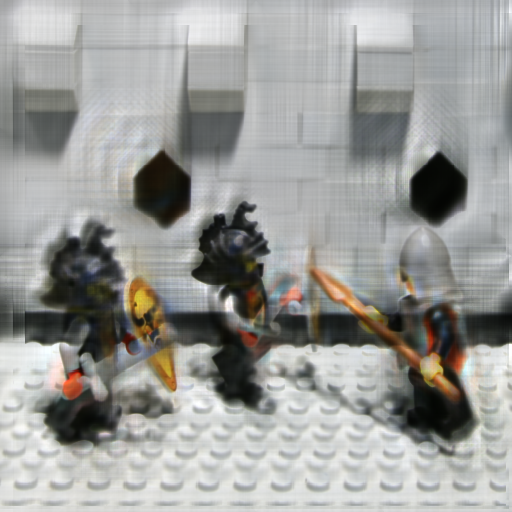
\includegraphics[width = 3.75cm]{../Figures/depth_compression/baseline_unscaled/Reconstruction_of_view_(9,9).png}};
			\end{scope}	
		\end{tikzpicture}
	};
	\draw[red] (box1.south east) rectangle (box1.north west);
	
	% Magnification box 2
	\node[anchor = north west, xshift = 0.1cm, inner sep = 0pt, outer sep = 0pt, scale = 1.825] (box2) at (I.north east) {
		
		\begin{tikzpicture}
			\begin{scope}
				\clip(A2) rectangle ++(S2);
				\node[anchor = center, inner sep = 0pt] (I) at (0, 0) {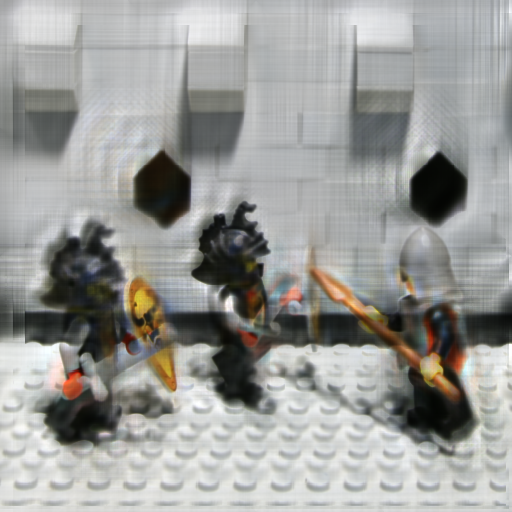
\includegraphics[width = 3.75cm]{../Figures/depth_compression/baseline_unscaled/Reconstruction_of_view_(9,9).png}};
			\end{scope}	
		\end{tikzpicture}
	};
	\draw[blue] (box2.south east) rectangle (box2.north west);
			
	
	\end{tikzpicture}
\end{document}
